\documentclass[12pt,a4paper]{report}
\usepackage[utf8]{inputenc}
\usepackage[english,russian]{babel}
\usepackage{indentfirst}
\usepackage{pdfpages}
\usepackage{titlesec}
\usepackage{listings}
\usepackage{amsmath}

% Вставка картинки
\usepackage{graphicx}
\graphicspath{{schemes/}}
\DeclareGraphicsExtensions{.pdf,.png,.jpg}

\usepackage[tableposition=top,singlelinecheck=false]{caption}

\usepackage[14pt]{extsizes}

\newcommand{\hsp}{\hspace{20pt}}
\titleformat{\chapter}[hang]{\large\bfseries}{\thechapter{. }}{0pt}{\large\bfseries}
\titlelabel{hlabel-formati}
\titlespacing{\chapter}{42pt}{-20pt}{12pt}
\titleformat{\section}[hang]{\large\bfseries}{\thesection{. }}{0pt}{\large\bfseries}
\titlespacing{\section}{42pt}{12pt}{5pt plus 5pt}

% Отступ абзаца
\usepackage{indentfirst}
\setlength{\parindent}{1.5cm}

% Межстрочный интервал
\usepackage{setspace}
\onehalfspacing % интервал 1.5


\usepackage{csvsimple}

\bibliography{biblio}
\lstset{frame=none, tabsize=4}

\usepackage[left=3cm, right=1cm, top=2cm, bottom=2cm]{geometry}

\AtBeginDocument{%
	\renewcommand\contentsname{Содержание}
}

\begin{document}
	% Титульник
	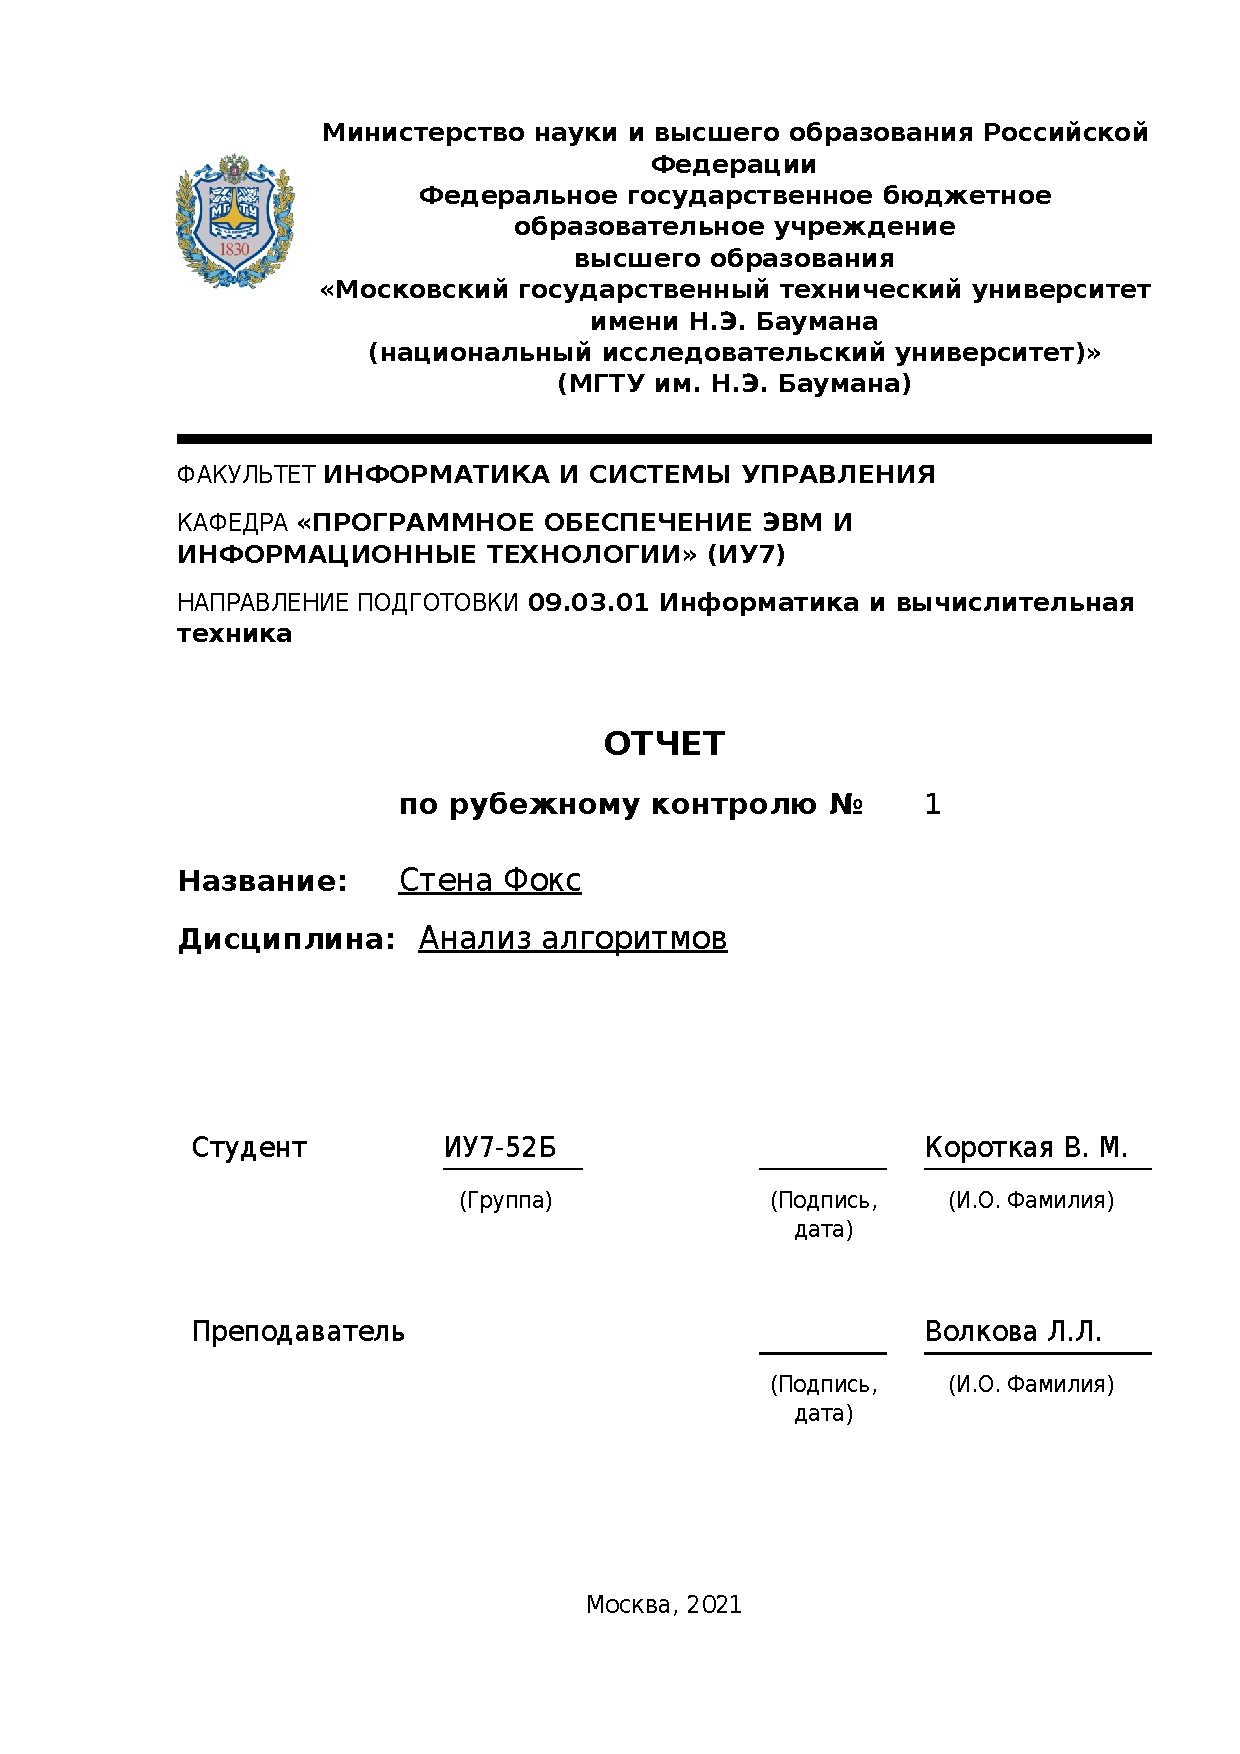
\includepdf[pages=1]{titul.pdf}
	% Оглавление
	\tableofcontents
	
	
	\newpage
	\chapter*{Введение}
	\addcontentsline{toc}{chapter}{Введение}
	
	\newpage
	\chapter{Аналитическая часть}
	
В данном разделе будет описана задача решаемая в данной работе.
	
\section{Стена Фокса}
	
	Решая задачу построения «стены Фокса», можно разбить
	стену на равные по длине участки и поручить постройку каждого участка отдельному каменщику. В этом случае все каменщики могут начать работу одновременно, укладывая нижний слой кирпичей (рис.
	1.1). Перед укладыванием очередного слоя каждому каменщику следует убедиться, что кирпичи предыдущего слоя уложены не только на
	его участке, но и на прилегающих участках. Если работа на соседних
	участках еще не закончена, возникают вынужденные паузы, связанные
	с синхронизацией работ на соседних участках. Отметим, что паузы
	могут возникать, даже если каменщики работают с одинаковой скоростью, поскольку объем работ, вообще говоря, зависит от номера участка, например он разный для крайних и внутренних частей стены.
	Можно сделать вывод о том, что эффективность организации
	параллельной работы будет тем выше, чем длиннее участки стены, и
	при достаточно длинных участках следует ожидать эффективности,
	близкой, но все же меньшей 1. При коротких участках стены (очень
	много каменщиков) эффективность будет невысокой, поскольку время
	независимой работы каждого каменщика будет невелико, они будут
	много времени проводить в ожидании друг друга на стыках участков.
	Отметим, что этот метод организации работы эффективен,
	даже если стена не очень высокая. Главным фактором, определяющим
	эффективность, является ее достаточная протяженность, по отношению к числу задействованных каменщиков.
	
	
	
	
	\begin{figure}[h!]
		\center{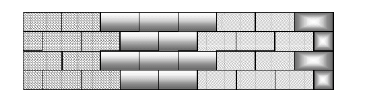
\includegraphics[scale=0.9]{anWall.png}}
		\caption{Визуализация работы каменщиков.}
		\label{fig:image}
	\end{figure}
	
\section*{Вывод}	

В данном разделе была рассмотрена задача "Стена Фокса".



\newpage
\chapter{Конструкторска часть}

В данном разделе будут разработаны схемы алгоритмов, реализующих стену Фокса.


\section{Схемы}



\begin{figure}[h!]
	\center{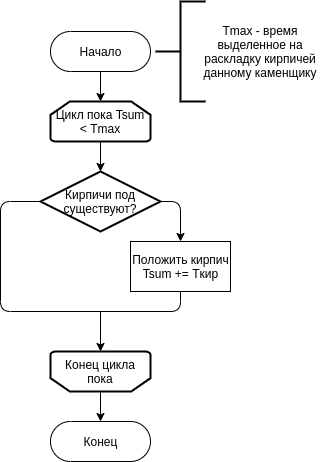
\includegraphics[scale=0.6]{bricllayer.png}}
	\caption{Схема работы одного каменщика.}
	\label{fig:image}
\end{figure}


\begin{figure}[h!]
	\center{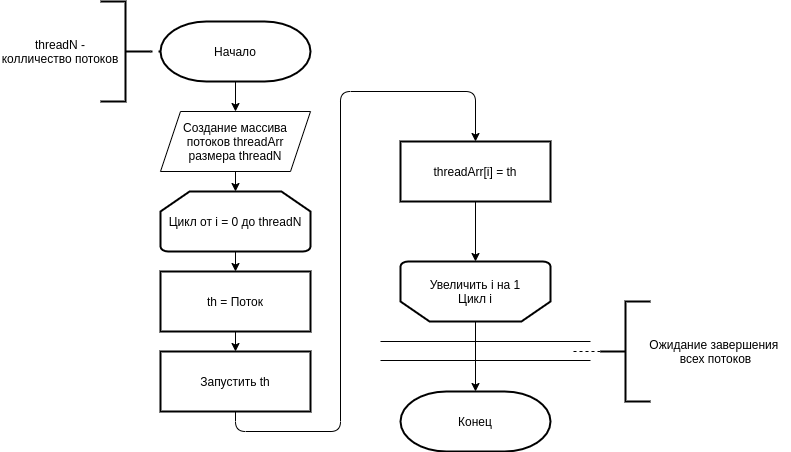
\includegraphics[scale=0.5]{parall.png}}
	\caption{Схема создания каменщиков в разных потоках.}
	\label{fig:image}
\end{figure}

%\section{Описание структур данных}

Для реализации визуализации стены Фокса, введем пользовательские типы данных:
\begin{itemize}
	\item struct wall - 
	\begin{itemize}
		\item brickWall - булевая матрица, описывающая существование кирпича на определенном участке;
		\item border - массив, описывающий границы работы каменщиков;
	\end{itemize}
	
	\item struct bricklayer -
	\begin{itemize}
		\item number - номер каменщика;
		\item countBrick - количество положенных кирпичей;
		\item speed - скорасть работы каменщика;
	\end{itemize}
\end{itemize}



\section*{Вывод}
На основании теоритических данных были построены схемы алгоритмов.

Так же приведено описание пользовательских структур данных.



\newpage
\chapter{Технологическая часть} 

В данном разделе приведены средства реализации и листинги кода.



\section{Средства реализации}
В качестве языка программирования был выбран с++. Данный язык знаком и предостовляет все необходимые ресурсы.
В качестве среды разработки я использовала Visual Studio Code, т.к. считаю его достаточно удобным и легким.
Visual Studio Code подходит не только для  Windows, но и для Linux, это еще одна причина, по которой я выбрала VS code, т.к. у меня установлена ОС  fedora 34.


\section{Сведенья о модулях программы}

Данноя программа разбита на модули:

\begin{itemize}
	\item main.cpp - файл, содержащий точку входа в программу;
	\item MainWindow.cpp - файл, содержащий реализацию алгоритмов.
\end{itemize}



\section{Реализация}

\noindent\textrm{Листинг 3.1: Функция запускающая конвейер.}
\begin{lstlisting}[frame=single, numbers=left]
	
\end{lstlisting}


\noindent\textrm{Листинг 3.1: Функция запускающая конвейер.}
\begin{lstlisting}[frame=single, numbers=left]
void MainWindow::brickparallel(QPainter &painter)
{
    std::vector<std::thread> threadArray;
    int start;
    int end;
	
    QVector<QBrush> color = 
    {QBrush(Qt::red, Qt::SolidPattern),
     QBrush(Qt::darkCyan, Qt::SolidPattern), 
     QBrush(Qt::green, Qt::SolidPattern),
     QBrush(Qt::yellow, Qt::SolidPattern) };
	
    for (int i = 0; i < 4; i++)
    {
        start = wall.border[i][0];
        end = wall.border[i][1];
        painter.setBrush(color[i]);
        threadArray.push_back
        (std::thread(&MainWindow::bricklayer, this, start,
         end, std::ref(brickl), i, std::ref(painter),
          color[i]));
    }
	
    for (int i = 0; i < 4; i++)
    {
        threadArray[i].join();
    }
}	
\end{lstlisting}


\noindent\textrm{Листинг 3.1: Функция реализующая каменщика.}
\begin{lstlisting}[frame=single, numbers=left]
void MainWindow::bricklayer(int start, int end, 
Bricklayer brick[],  int num, QPainter &painter, 
QBrush color)
{
	const int delay_value = 1;
	
	int time = 0;
	
	int row = (end - start)/deltaBrick;
	int column = 1;
	int delta = 0;
	int x = 0;
	int y = 0;
	bool flag;
	int wait = 1;
	int i = 0;
	
	int blok = 1500;
	
	while (time < blok)
	{
		i++;
		row--;
		x = start + deltaBrick * (row) + delta;
		y = y_max - deltaBrick/2 * column;
		flag = (wall.brickWall[column - 1][x/25]* 
		wall.brickWall[column - 1][x/25 + 1]);
		if ( (  flag ) && !(wall.brickWall[column][x/25]) && 
		!( wall.brickWall[column][x/25 + 1] )) {
			mtx1.lock();
						
			painter.setBrush(color);
			painter.drawRect(x, y, deltaBrick, deltaBrick/2);
						
			wall.brickWall[column][x/25] = 1;
			wall.brickWall[column][x/25 + 1] = 1;
			mtx1.unlock();
			
			
			mtx2.lock();
			displayImage();
			mtx2.unlock();
			
			wait = (rand()%20 + 1 ) * brickl[num].speed;
			time += wait;
			
			delay(delay_value * wait);
			brickl[num].countBrick++;
		}
		else
		{
			i--;
		}
		if (!row) {
			row = (end - start)/deltaBrick;
			column++;
		}
		if (column % 2)
		delta = 0;
		else
		delta = 25;		
	}
}
\end{lstlisting}

	
\section*{Вывод}
В данном разделе был реализован выше описанный алгоритм шифрования. Разработано программное обеспечение, представленны листинги программы.



\newpage
\chapter{Исследовательская часть} 


В данном разделе будет приведена работа программы.



\newpage
\chapter*{Заключение}
\addcontentsline{toc}{chapter}{Заключение}


	
	\newpage
	\renewcommand\bibname{Список литературы}
	\addcontentsline{toc}{chapter}{Список литературы}
	\makeatletter % список литературы
	\def\@biblabel#1{#1. }
	\makeatother
	\begin{thebibliography}{2}
		\bibitem{analyse_info} Дж. Макконнел. Анализ алгоритмов. Активный обучающий подход. -- М.: Техносфера, 2017. -- 267с.
		\bibitem{anatyse_info}Основы программирования на языках Си и C++ для начинающих[Электронный ресурс]. Режим доступа: http://cppstudio.com/ (дата обращения 10.10.2021)
		\bibitem{analyse_info}LINUX.ORG.RU - Русскоязычная информация о ОС Linux[Электронный ресурс] Режим доступа://www.linux.org.ru/(дата обращения 25.10.2021)
		\bibitem{analyse_info}  Документация языка C++ 98 [Электронный ресурс], режим доступа: http://www.open-std.org/JTC1/SC22/WG21/ (дата обращения 10.12.2021)
		\bibitem{} Р.А. Волков, А.Н. Гнутов, В.К. Дьячков и др. Конвейеры. Справочник. -Машиностроение, Ленинградское отделение, 1984.
		
	\end{thebibliography}
	
\end{document}